\documentclass[a4paper]{jsarticle}
\usepackage{otf}
\usepackage[dvips]{graphicx}
\usepackage{amsmath,amssymb}
\usepackage{fancyheadings}
\usepackage{enumerate}
\usepackage{ascmac}
\usepackage{color}
\usepackage{listings, jlisting}
\usepackage{float}
%\usepackage{footmisc}
\lhead{「数値計算」(CSプログラム) 第14回 演習}
\chead{}
\rhead{\thepage}
\pagestyle{fancy}
\cfoot{}
\addtolength{\textheight}{40pt}
\setlength{\headsep}{10pt}
\setlength{\voffset}{-10pt}
\setlength{\topmargin}{-30pt}
\lstset{% 
language={C}, 
backgroundcolor={\color[gray]{.85}},% 
basicstyle={\footnotesize\ttfamily},% 
identifierstyle={\footnotesize\ttfamily},% 
commentstyle={\footnotesize\ttfamily \color[rgb]{0.5,0.5,0.5}},% 
keywordstyle={\footnotesize\ttfamily \color[rgb]{0,0,0}},% 
ndkeywordstyle={\footnotesize\ttfamily},% 
stringstyle={\footnotesize\ttfamily}, 
frame={tb}, 
breaklines=true, 
columns=[l]{fullflexible},% 
%numbers=left,% 
numbers=none,% 
xrightmargin=0zw,% 
xleftmargin=3zw,% 
numberstyle={\scriptsize},% 
stepnumber=1, 
numbersep=1zw,% 
escapechar={\^},%
morecomment=[l]{//}% 
} 
\def\TODO{\textbf{\LARGE TODO: }}
\def\Ctrl{\texttt{Ctrl}}
\def\zaki{\CID{14290}}
\title{「数値計算」(CSプログラム) 第14回 演習}
\author{2311081 木村 慎之介}
\date{2025年1月30日}
\begin{document}
\maketitle

\section*{演習 1: オイラー法の動作確認}
\subsection*{課題 1: 誤差の評価}
まず作成したコードを以下に載せる。
\lstinputlisting[caption={\texttt{1階微分方程式を解くプログラム}},numbers=left, label=source_euler]{../calculation/euler.c}
\hspace{1em}このプログラムはsolve\_deという関数と65行目から70行目の繰り返し処理で区間を\(1/10\)ずつ小さくしたときの誤差を出力している。
他の行のコードに関してはホイン法とルンゲクッタ法に関するコードなので課題3にて説明する。
このプログラムを実行したときのオイラー法による解法の出力を以下に載せる。

\begin{lstlisting}[caption={{\texttt{オイラー法による解法の誤差の出力}}}, numbers=left, label=soure_euler_result]
  --- euler ---
  h = 0.10000
  result: 2.593742
  error = 0.1245393684
  h = 0.01000
  result: 2.704814
  error = 0.0134679990
  h = 0.00100
  result: 2.716924
  error = 0.0013578962
  h = 0.00010
  result: 2.718146
  error = 0.0001359016
  -----
\end{lstlisting}

この結果から区間の幅を\(1/10\)するごとに誤差の値も\(1/10\)になることが確かめられる。
\subsection*{課題 2: 2階常微分方程式の数値解法}
まず2階微分方程式を解くプログラムをいかに載せる。
\lstinputlisting[caption={\texttt{2階微分方程式を解くプログラム}}, numbers=left, label=source_second_euler]{../calculation/pendulum.c}
\hspace{1em}次にコード\ref{source_second_euler}の説明を行う。
まず、solve\_second\_de関数では連立方程式を利用して2階分方程式をステップごとに計算して数値解を求めている。
もとめた数値解はdatファイルに保存して、gnuplotでグラフを描画しやすいようにしている。
すべてのステップで計算が終わったらcでgnuplotを呼び出してdatファイルに保存したデータを\(t\)-\(x\)グラフにプロットしてpngファイルとして出力する。
また、main関数では区間を変えながら繰り返し処理を行いsolve\_second\_deを呼び出して各区間幅に関して数値解のグラフを出力している。
\hspace{1em}以上のコードを実行して得た各区間幅に対する数値解のグラフを以下に載せる。

\begin{figure}[H]
  \centering
  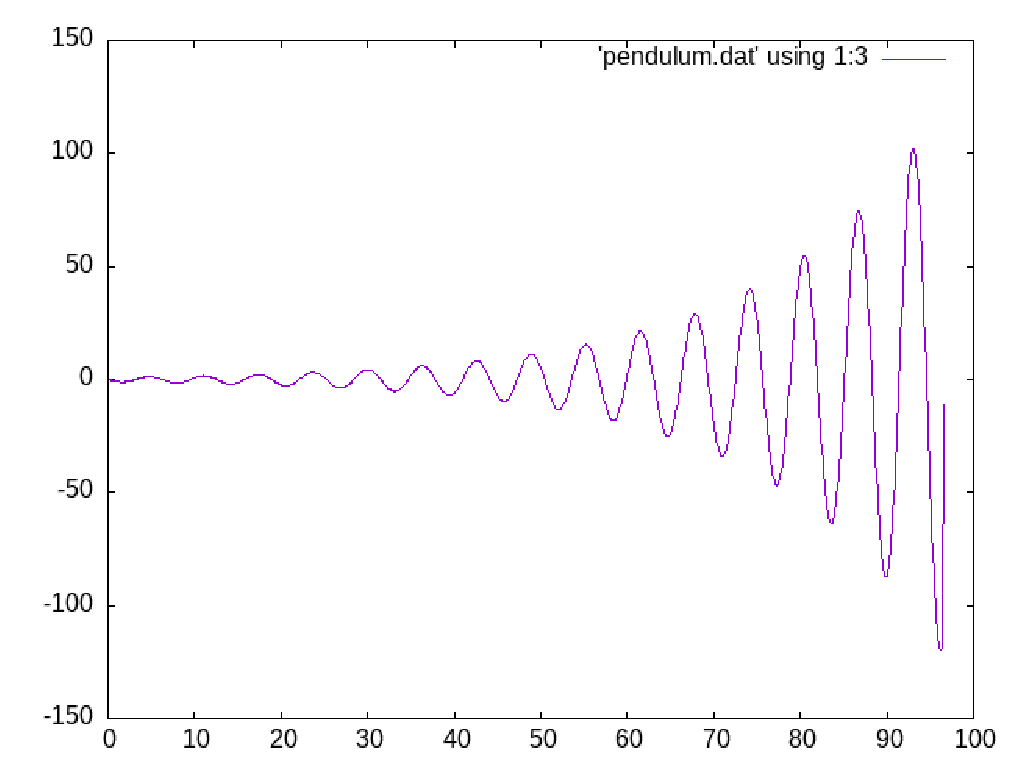
\includegraphics[width=0.8\textwidth]{pictures/pendulum1.eps}
  \caption{\(\text{interval} = 0.1\)の時の数値解のグラフ}
  \label{figure_pendulum1}
\end{figure}

\begin{figure}[H]
  \centering
  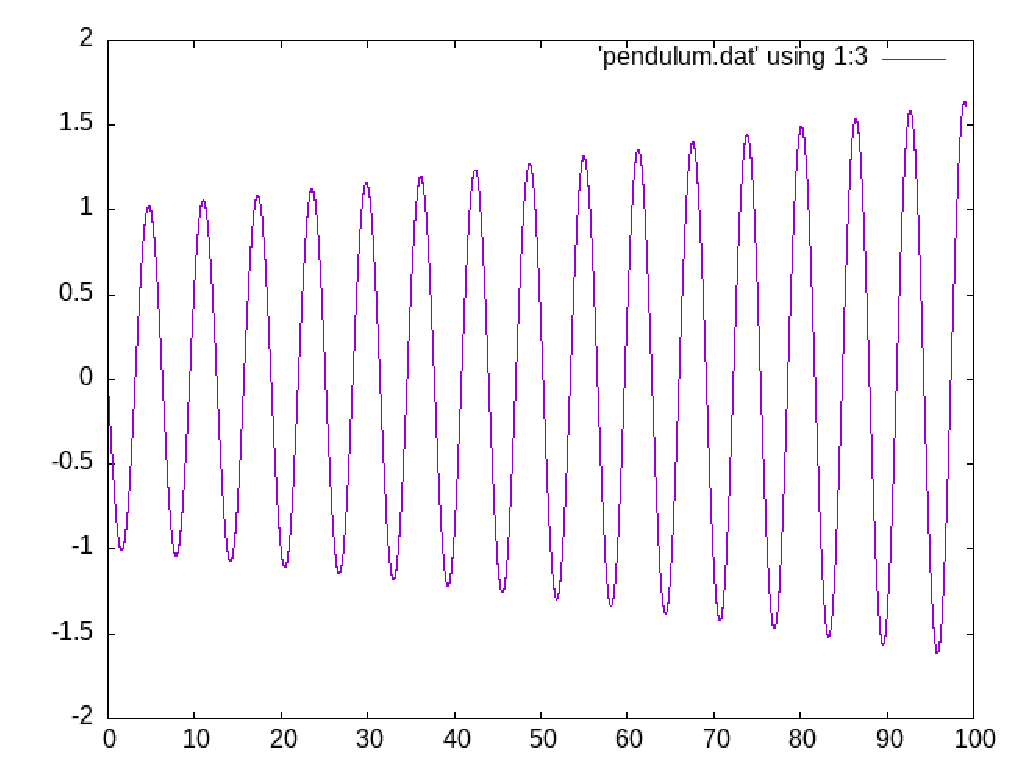
\includegraphics[width=0.8\textwidth]{pictures/pendulum2.eps}
  \caption{\(\text{interval} = 0.01\)の時の数値解のグラフ}
  \label{figure_pendulum2}
\end{figure}

\begin{figure}[H]
  \centering
  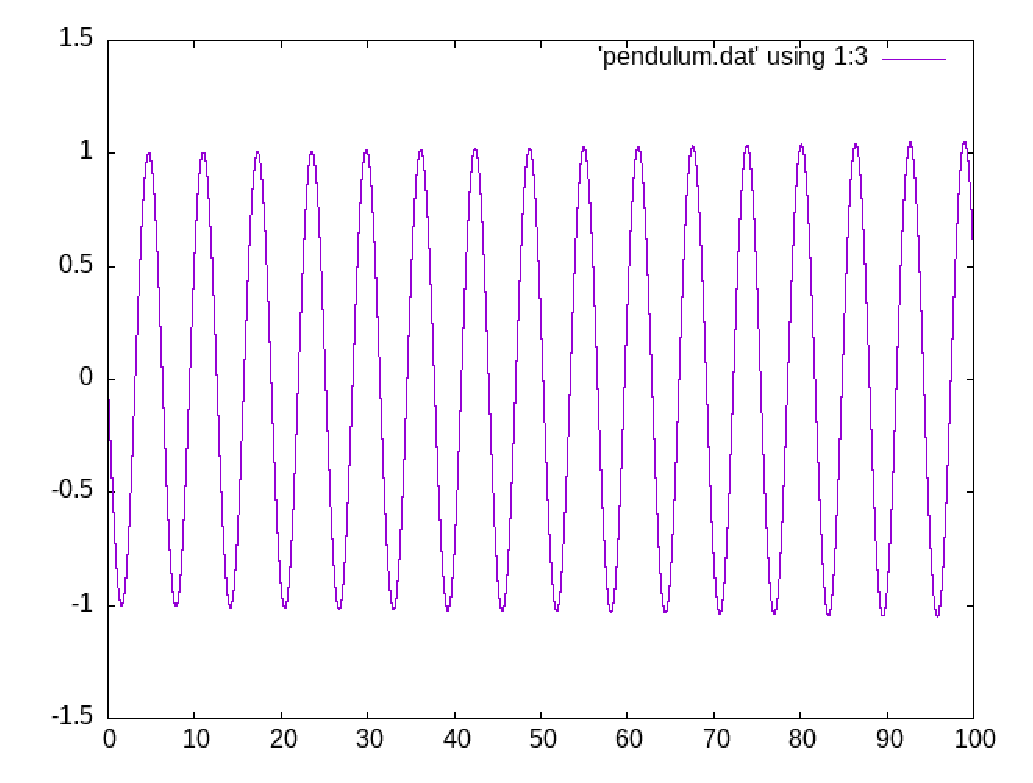
\includegraphics[width=0.8\textwidth]{pictures/pendulum3.eps}
  \caption{\(\text{interval} = 0.001\)の時の数値解のグラフ}
  \label{figure_pendulum3}
\end{figure}

\begin{figure}[H]
  \centering
  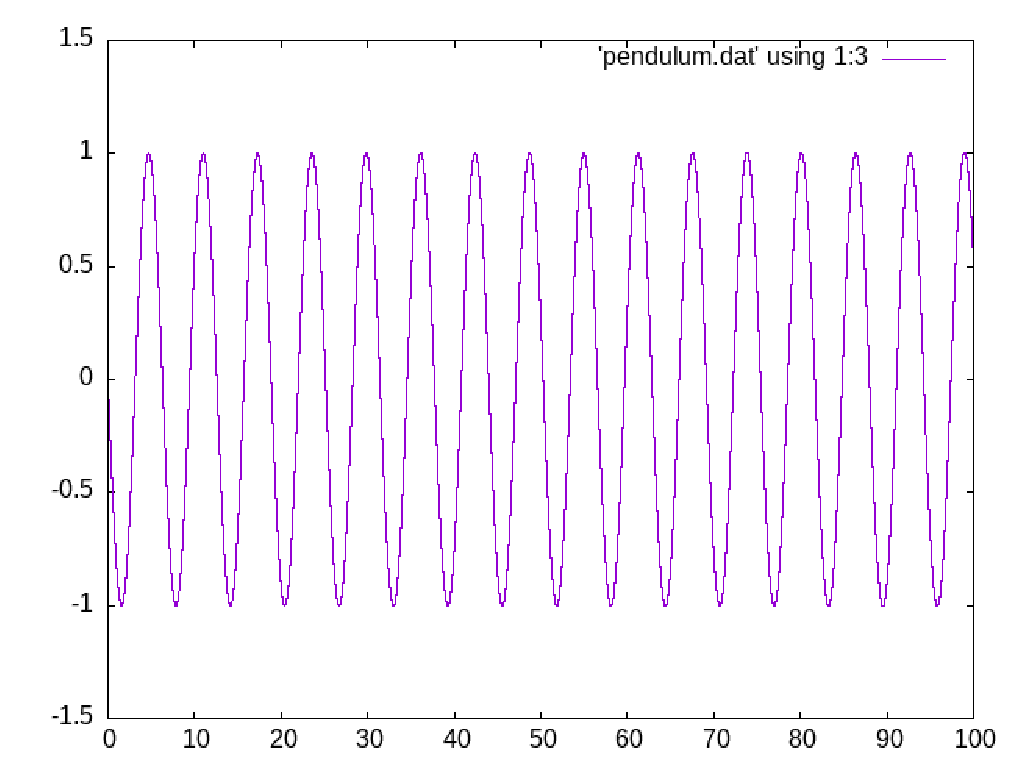
\includegraphics[width=0.8\textwidth]{pictures/pendulum4.eps}
  \caption{\(\text{interval} = 0.0001\)の時の数値解のグラフ}
  \label{figure_pendulum4}
\end{figure}

以上のグラフを確認すると区間幅が大きい時は振幅が大きくなりながら振動するグラフを得たが、区間幅が小さくなるにつれて振幅の変化が徐々に小さくなって正弦波に収束していった。

\section*{演習 3: ホイン法・ルンゲクッタ法}
\subsection*{課題 3}
ホイン法とルンゲクッタ法のコードはコード\ref{source_euler}に記した。
まずはホイン法のプログラムとその出力の説明を行う。 \\
\hspace{1em}ホイン法のプログラムはsolve\_de\_heun関数で実装した。
基本的な実装方針はオイラー法と変わらないが、解の更新を行う際に1ステップ先の解と2ステップ先の解の平均をとり、それを次ステップの解とした。
区間幅ごとのホイン法による解の誤差の出力は以下のようになった。

\begin{lstlisting}[caption={\text{ホイン法の出力}}, numbers=left, label=result_heun]
  --- heun ---
  h = 0.10000
  result: 2.714081
  error = 0.0042009819
  h = 0.01000
  result: 2.718237
  error = 0.0000449659
  h = 0.00100
  result: 2.718281
  error = 0.0000004527
  h = 0.00010
  result: 2.718282
  error = 0.0000000045
  -----
\end{lstlisting}

次にルンゲクッタ法の説明を行う。
ルンゲクッタ法のコードはコード\ref{source_euler}のsolve\_de\_runge\_kutta関数の部分に当たる。
こちらも基本方針はオイラー法と同じで、nステップ目の数値回を求めるのに4つ先のステップの値を利用している点がホイン法との違いである。
区間幅を\(0.1\)から\(0.0001\)へ\(10^{-1}\)倍していきながら変えていったときのルンゲクッタ法による解の誤差の出力は以下のようになった。

\begin{lstlisting}[caption={\texttt{ルンゲクッタ法の誤差の出力}}]
  --- runge kutta ---
  h = 0.10000
  result: 2.718280
  error = 0.0000020843
  h = 0.01000
  result: 2.718282
  error = 0.0000000002
  h = 0.00100
  result: 2.718282
  error = 0.0000000000
  h = 0.00010
  result: 2.718282
  error = 0.0000000000
  -----
\end{lstlisting}

以上の結果を見ると、ホイン法では誤差が\(10^{-2}\)倍しているため2次収束を、ルンゲクッタ法では誤差が\(10^{-4}\)倍しているため4次収束をしていることがわかる。

\end{document}
